%%%%%%%%%%%%%%%%%%%%%%%%%%%%%%%%%%%%%%%%%%%%%%%%%%%%%%%%%%%%%%%%%%%%%%
% Lớp 11 | Hàm số lượng giác và phương trình lượng giác | Hàm số lượng giác và đồ thị
% Dạng 1D1?4-3: Xét tính đơn điệu
% Số câu: 9  (sinh tự động bởi tach_cau.py; từ nay thầy sửa trực tiếp file này)
%%%%%%%%%%%%%%%%%%%%%%%%%%%%%%%%%%%%%%%%%%%%%%%%%%%%%%%%%%%%%%%%%%%%%%

%%%%%%%%%%%%%%%% TRẮC NGHIỆM 4 PHƯƠNG ÁN %%%%%%%%%%%%%%%%

% nguồn: Ok_TracNghiemLop11_Lan1
\begin{ex}%[1D1N4-3]%[ma:c63001e7]
	Xét hàm số $y=\sin x$ trên đoạn  $\left[-\pi;0 \right]$. Khẳng định nào sau đây là đúng?
	\choice 
		{\True Hàm số đã cho nghịch biến trên đoạn $\left[-\pi;-\dfrac{\pi }{2} \right]$;  đồng biến trên đoạn $\left[-\dfrac{\pi }{2};0 \right]$}
		{Hàm số đã cho nghịch biến trên các đoạn $\left[-\pi;-\dfrac{\pi }{2}  \right]$ và $\left[-\dfrac{\pi }{2};0 \right]$}
		 {Hàm số đã cho đồng biến trên các đoạn $\left[-\pi;-\dfrac{\pi }{2} \right]$ và $\left[-\dfrac{\pi }{2};0 \right]$}
		{Hàm số đã cho đồng biến  trên đoạn $\left[-\pi;-\dfrac{\pi }{2} \right]$; nghịch biến trên đoạn $\left[-\dfrac{\pi }{2};0 \right]$}
	 \loigiai{
		Ta có  bảng biến thiên của hàm số $y=\sin x$ trên đoạn $\left[-\pi;\pi \right]$.
		\begin{center}
			\begin{tikzpicture}[font=\normalsize]
					 \tkzTabInit[espcl=2]
						 {$x$ /1,$g (x)$/2}
						{$-\infty$,$-1$,$1$,$2$,$+\infty$} 
					 \tkzTabVar{+/$0$,-/$-1$,R /,+/$1$,-/$0$}
					 \tkzTabIma{2}{4}{3}{$0$}
				\end{tikzpicture}
		\end{center}
	Khi đó, hàm số  nghịch biến trên đoạn $\left[-\pi;-\dfrac{\pi }{2} \right]$; đồng biến trên đoạn $\left[-\dfrac{\pi }{2};0 \right]$.}
\end{ex}

% nguồn: Ok_TracNghiemLop11_Lan1
\begin{ex}%[1D1N4-3]%[ma:ccb68cba]
	 Hàm số $y=\tan x$ đồng biến trên khoảng
	 \choice
		 {$\left(-\pi;0\right)$}
		{$\left(0;\pi \right)$} 
		 {\True $\left(\dfrac{\pi}{2};\pi \right)$}
		 {$\left(0;5\right)$}
	\loigiai{ 
		Tập xác định  $\mathscr{D}=\mathbb{R}\setminus \left\{\dfrac{\pi}{2}\right\}$.\\
	 Hàm số $y=\tan x$ đồng biến trên từng khoảng xác định nên nó đồng biến trên khoảng $\left(\dfrac{\pi}{2};\pi \right)$.}
\end{ex}

% nguồn: Ok_TracNghiemLop11_Lan1
\begin{ex}%[1D1N4-3]%[ma:d657cfaa]
	Hàm số  nào sau đây nghịch biến trên $\left( \dfrac{\pi }{2};\pi \right)$?
	\choice 
		{$y=-\sin x$} 
		{\True  $y=\cos x$}
		{$y=-\cot  x$}
		{$y=\tan x$} 
	\loigiai{ 
		Với $x\in \left( \dfrac{\pi }{2};\pi \right)$,  khi giá trị của $x$ tăng thì giá trị tương ứng của hàm số $y=\cos x$ giảm.\\
	$\Rightarrow $ Hàm số $y=\cos x$  nghịch biến trên $\left( \dfrac{\pi }{2};\pi \right)$.}
\end{ex}

% nguồn: Ok_TracNghiemLop11_Lan1
\begin{ex}%[1D1N4-3]%[ma:669a3877]
	Tìm mệnh đề đúng. 
	 \choice
		{Hàm số $y=\cot x$  đồng biến trên khoảng $\left( 0;\pi \right)$}
		{\True Hàm số $y=\sin x$ đồng biến trên khoảng $\left( \dfrac{3\pi  }{2};\dfrac{5\pi }{2} \right)$}
		{Hàm số $y=\sin x$ nghịch  biến trên khoảng $\left( \pi;2\pi \right)$}
		{Hàm số $y=\cos x$ nghịch biến trên khoảng  $\left( -\dfrac{\pi }{2};\dfrac{\pi }{2} \right)$}
	\loigiai{Hàm số $\sin x$ đồng biến trên các khoảng $\left(-\dfrac{\pi}{2}+k2\pi;\dfrac{\pi}{2}+k2\pi\right)(k\in \mathbb{Z})$.} 
\end{ex}

% nguồn: Ok_TracNghiemLop11_Lan1
\begin{ex}%[1D1H4-3]%[ma:be2b7dde]
	Phương trình $\sin  x = -\dfrac{\sqrt{3}}{2}$ có nghiệm là
	\choice 
		{$\hoac{&x = - \frac{\pi}{3}  + 2\pi \\& x = \frac{\pi}{3} + 2\pi}$}
		{$\hoac{&x  = - \frac{\pi}{3} + k2\pi \\& x = \frac{2 \pi}{3} + k2\pi}$}
		{\True $\hoac{&x = -  \frac{\pi}{3} + k2\pi \\& x = \frac{4 \pi}{3} + k2\pi}$}
		{$\hoac{&x  = - \frac{\pi}{3} + k\pi \\& x = \frac{4 \pi}{3} + k\pi}$}
	\loigiai{Ta có $$\sin x = -\dfrac{\sqrt{3}}{2} \Leftrightarrow \sin x  = \sin \left(- \frac{\pi}{3}\right)\Leftrightarrow \hoac{&x = - \frac{\pi}{3} + k2\pi \\& x = \frac{4 \pi}{3} + k2\pi.}$$
		Vậy nghiệm của phương trình là $\hoac{&x =  - \frac{\pi}{3} + k2\pi \\& x = \frac{4 \pi}{3} + k2\pi.}$
	} 
\end{ex}


%%%%%%%%%%%%%%%% ĐÚNG/SAI %%%%%%%%%%%%%%%%

% nguồn: Ok_dungsai_lop11_Lan1
\begin{ex}%[1D1N4-3]%[ma:7bdb59aa]
 \immini{ 
 Trên khoảng $(-\pi;\pi)$, đồ thị của hàm số $y=\sin x$ được cho như hình vẽ bên. Mỗi khẳng định sau đây đúng  hay sai?
  \choiceTF
  {Hàm  số $y=\sin x$ nghịch biến trên khoảng $(-\pi;0)$}
  {\True Hàm số $y=\sin x$ đồng biến  trên khoảng $\left(-\dfrac{\pi}{2};\dfrac{\pi}{2}\right)$}
  {\True Hàm số $y=\sin x$ nghịch biến trên khoảng $\left(\dfrac{\pi}{2};\pi\right)$} 
  {Hàm số $y=\sin x$ đồng biến trên khoảng$(0;\pi)$} 
   }{
  \begin{tikzpicture}[scale=0.8,font=\footnotesize,line join=round,line cap=round,>=stealth]
    \draw[->] (-4,0)  -- (4,0) node[below] {$x$};
    \draw[->] (0,-2) -- (0,2) node[right] {$y$}; 
     \node at (0,0) [below right]{$O$};
    \draw[thick,samples=100,domain=-pi:pi] plot  (\x,{sin ((\x)*180/pi)});
    \draw[dashed] (0,1) node[left] {$1$} -- (1.57,1) -- (1.57,0)  node[below] {$\tfrac{\pi}{2}$};
    \draw[dashed] (0,-1) node[right] {$-1$} -- (-1.57,-1)  -- (-1.57,0) node[above] {$-\tfrac{\pi}{2}$};
    \fill (1.57,1) circle (1pt); 
    \fill  (-1.57,-1) circle (1pt);
     \node at (3.14,0) [below]{$\pi$};
    \node at  (-3.14,0) [above]{$-\pi$};
   \end{tikzpicture}
   }
  \loigiai{
  \begin{itemchoice}
   \itemch hàm số $y=\sin x$ nghịch biến trên khoảng $\left(-\pi;-\dfrac{\pi}{2}\right)$ và đồng biến trên khoảng $\left(-\dfrac{\pi}{2};\pi\right)$. 
   \itemch Hàm số  $y=\sin x$ đồng biến trên khoảng $\left(-\dfrac{\pi}{2};\dfrac{\pi}{2}\right)$.
   \itemch Hàm số $y=\sin  x$ nghịch biến trên khoảng $\left(\dfrac{\pi}{2};\pi \right)$.
   \itemch Hàm số $y=\sin  x$ đồng biến trên khoảng $\left(0; \dfrac{\pi}{2}\right)$ và nghịch biến trên khoảng $\left(\dfrac{\pi}{2};\pi \right)$.
  \end{itemchoice}
 } 
\end{ex}

% nguồn: Ok_dungsai_lop11_Lan1
\begin{ex}%[1D1N4-3]%[ma:671242bd]
 Mỗi khẳng  định sau đây đúng hay sai?
 \choiceTF 
  {\True Hàm số $y=\sin  x$ đồng biến trên khoảng $\left(0;\dfrac{\pi}{2}\right)$}
  {Hàm số $y=\cos x$ đồng biến trên  khoảng $\left(0;\dfrac{\pi}{2}\right)$}
  {\True Hàm số $y=\tan  x$ đồng biến trên khoảng $\left(0;\dfrac{\pi}{2}\right)$}
  {Hàm số $y=\cot x$ đồng  biến trên khoảng $\left(0;\dfrac{\pi}{2}\right)$}
 \loigiai{ 
  Theo  lý thuyết, ta có
  \begin{itemchoice}
   \itemch Hàm số $y=\sin  x$ đồng biến trên khoảng $\left(0;\dfrac{\pi}{2}\right)$.
   \itemch Hàm số $y=\cos x$ nghịch biến trên khoảng  $\left(0;\dfrac{\pi}{2}\right)$.
   \itemch Hàm số $y=\tan x$  đồng biến trên khoảng $\left(0;\dfrac{\pi}{2}\right)$.
   \itemch Hàm  số $y=\cot x$ nghịch biến trên khoảng $\left(0;\dfrac{\pi}{2}\right)$.
  \end{itemchoice}
  }
\end{ex}

% nguồn: Ok_dungsai_lop11_Lan2
\begin{ex}%[1D1H4-3]%[ma:58824536]
	Cho các hàm số sau $f(x)=\sin  x$ và $g(x)=\cos x$. Khi đó
	 \choiceTF{\True Hàm số $f(x)=\sin x$ đồng biến trên khoảng $\left(-\dfrac{\pi}{2}; \dfrac{\pi}{2}\right)$}
		{\True Hàm số $f(x)$ nghịch biến trên khoảng  $\left(\dfrac{3\pi}{4}; \dfrac{5\pi}{4}\right)$}
		{\True Hàm số  $g(x)$ nghịch biến trên khoảng $(0; \pi)$}
		{Hàm số $g(x)$  đồng biến trên khoảng $\left(\dfrac{25\pi}{6}; \dfrac{13\pi}{3}\right)$}
	 \loigiai{
		\begin{itemchoice}
			 \itemch \textbf{Đúng.}\\
			Hàm số $f(x)=\sin x$ đồng biến trên khoảng  $\left(-\dfrac{\pi}{2}; \dfrac{\pi}{2}\right)$.
			\itemch  \textbf{Đúng.}\\
			Vì $\left(\dfrac{3\pi}{4}; \dfrac{5\pi}{4}\right)\subset \left(\dfrac{\pi}{2}; \dfrac{3\pi}{2}\right)$ nên hàm số $f(x)$ nghịch biến trên  khoảng $\left(\dfrac{3\pi}{4}; \dfrac{5\pi}{4}\right)$.
			\itemch  \textbf{Đúng.}\\
			Hàm số $g(x)=\cos x$ nghịch biến trên khoảng  $(0; \pi)$.
			 \itemch \textbf{Sai.}\\
			Vì $\dfrac{25\pi}{6}=\dfrac{\pi}{6}+4\pi, \dfrac{13\pi}{3}=\dfrac{\pi}{3}+4\pi$, đồng thời $\left(\dfrac{\pi}{6}; \dfrac{\pi}{3}\right)\subset \left(0; \dfrac{\pi}{2}\right)$ nên hàm số $g(x)=\cos x$ nghịch biến trên khoảng $\left(\dfrac{\pi}{6}; \dfrac{\pi}{3}\right)$, suy ra hàm số cũng nghịch biến trên khoảng  $\left(\dfrac{25\pi}{6}; \dfrac{13\pi}{3}\right)$.
		\end{itemchoice}
	 }
\end{ex}

% nguồn: Ok_dungsai_lop11_Lan2
\begin{ex}%[1D1H4-3]%[ma:c7dfb844]
	Đường cong trong hình dưới là đồ thị  hàm số $y=\cos x$.
	\begin{center}
		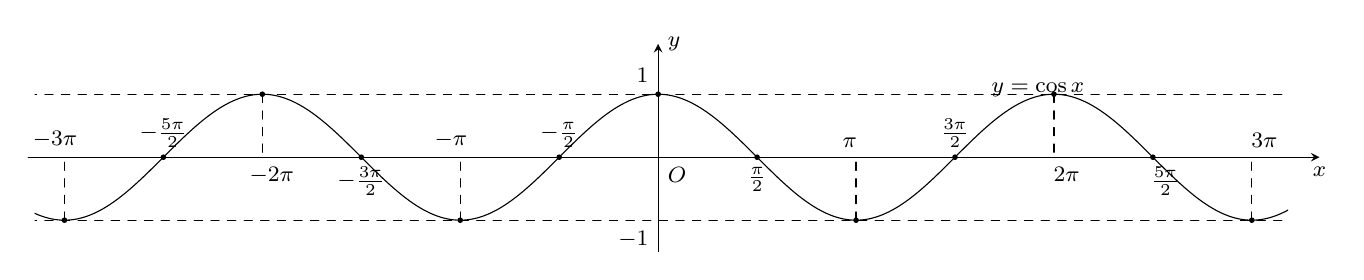
\begin{tikzpicture}[scale=0.8,>=stealth,font=\footnotesize,line join=round,line cap=round]
				 \def\xmin{-10} \def\xmax{10.5} \def\ymin{-1.5} \def\ymax{1.8}
				\draw[->] (\xmin,0)--(\xmax,0)  node [below]{$x$};
				\draw[->]  (0,\ymin)--(0,\ymax) node [right]{$y$};
				\node  at (0,0) [below right]{$O$};
				\clip (\xmin+0.1,\ymin+0.1)  rectangle (\xmax-0.5,\ymax-0.1);
				\draw[smooth,samples=400,domain=\xmin:\xmax] plot (\x,{cos  (\x r)});
				 \draw[dashed] (\xmin,1)--(\xmax,1)
					(\xmin,-1)--(\xmax,-1); 
				\foreach \x in  {-3*pi,-2.5*pi,-2*pi,-1.5*pi,-pi,-0.5*pi,0}
					{\draw[fill=black] (\x,cos \x*180/pi) circle (1pt); 
				\draw[dashed] (\x,cos  \x*180/pi)--(\x,0);
				\draw[fill=black] (-\x,cos  -\x*180/pi) circle (1pt);
				\draw[dashed] (-\x,cos \x*180/pi)--(-\x,0);} 
				 \node at (0,1.3) [left]{$1$};
				\node at (0,-1.3) [left]{$-1$}; 
				\node at  (-2*pi+0.15,0) [below]{$-2\pi$};
				\node at (-3*pi-0.15,0) [above]{$-3\pi$}; 
				 \node at (-2.5*pi,0) [above]{$-\frac{5\pi}{2}$};
				\node at  (-1.5*pi,0) [below]{$-\frac{3\pi}{2}$};
				\node at (-pi-0.15,0) [above]{$-\pi$}; 
				\node at  (-0.5*pi,0) [above]{$-\frac{\pi}{2}$};
				\node at  (0.5*pi,0) [below]{$\frac{\pi}{2}$};
				\node  at (pi-0.1,0) [above]{$\pi$};
				\node at  (1.5*pi,0) [above]{$\frac{3\pi}{2}$};
				\node  at (2*pi+0.2,0) [below]{$2\pi$};
				\node at  (2.5*pi+0.2,0) [below]{$\frac{5\pi}{2}$};
				\node at (3*pi+0.2,0) [above]{$3\pi$}; 
				\node at (1.6*pi+1,0.8)  [above]{$y=\cos x$};
			\end{tikzpicture}
	\end{center}
	 \choiceTF{Hàm số $y=\cos x$ đồng biến trên khoảng $\left(-\dfrac{\pi}{2}; \dfrac{\pi}{2}\right)$}
		{Hàm số  $y=\cos x$ nghịch biến trên khoảng $\left(-\dfrac{\pi}{2}; \dfrac{\pi}{2}\right)$}
		{\True Hàm số $y=\cos x$ đồng biến trên  khoảng $\left(-\dfrac{\pi}{2}; 0\right)$}
		{\True Hàm số $y=\cos  x$ nghịch biến trên khoảng $\left(0; \dfrac{\pi}{2}\right)$}
	\loigiai{ 
		\begin{itemchoice}
			\itemch \textbf{Sai.}\\ 
			Khoảng $\left(-\dfrac{\pi}{2}; \dfrac{\pi}{2}\right)$ chứa khoảng đồng biến và khoảng nghịch biến của hàm  số $y=\cos x$.
			\itemch \textbf{Sai.}\\  Khoảng $\left(-\dfrac{\pi}{2}; \dfrac{\pi}{2}\right)$ chứa khoảng đồng biến và khoảng nghịch biến của hàm số $y=\cos x$.
			\itemch  \textbf{Đúng.}\\
			 Hàm số $y=\cos x$ đồng biến trên khoảng $\left(-\dfrac{\pi}{2}; 0\right)$.
			\itemch \textbf{Đúng.}\\ 
			Hàm  số $y=\cos x$ nghịch biến trên khoảng $\left(0; \dfrac{\pi}{2}\right)$.
		\end{itemchoice}
	 }
\end{ex}
